\documentclass[12pt]{report}
\usepackage{scribe,graphicx,graphics,subcaption}


\course{MIT 9.520} 	
\coursetitle{Statistical Learning Theory}	
\semester{Fall 2014}
\lecturenumber{2}	
\lecturedate{}		


% Insert your name here!
\scribe{Brando Miranda}

\begin{document}


\maketitle

\paragraph{Problem 1}

\begin{proof}Let:

$$J(w) = \sum_{i=1}^n ( \left\langle w, x_i \right\rangle - y_i ) ^2 + 2\lambda  ||w||_1 = \sum_{i=1}^n ( \sum_{j=1}^d w_j x_i^j - y_i ) ^2 + 2\lambda \sum_{j=1}^d |w_j| $$

Lets take the partial sub gradient wrt to component $w_i$:

$$\partial J(w) = 2 \sum_{i=1}^n ( \sum_{j=1}^d w_j x_i^j - y_i ) x_i^k + 2\lambda h  = 0$$

where h is defined as follows:

\begin{displaymath}
   h = \left\{
     \begin{array}{lr}
       sign(w^k) & $if $ w^k \neq 0\\
       \in \left[-1, 1 \right] & $if $ w^k = 0
     \end{array}
   \right.
\end{displaymath} 

Further algebraic manipulation yields:

$$ \sum_{j=1}^d w_j\sum_{i=1}^n x_i^k x_i^j - \sum_{i=1}^n y_i  x_i^k + \lambda h  = 0$$

From the problem we know: $\sum_{i=1}^n x_i^j x_i^k  = \delta_{j,k}$ and $y^j = \sum_{i=1}^d x_i^j y_i$ 

Subsituting them to the above yields:

$$ w^k =  y^k - \lambda h $$

Now we proceed our analysis in two cases. 

Case 1: $w^k = 0 \implies h \in [-1,1]$

$$0 \in  y^k - \lambda \left[-1, 1 \right] $$

For the interval above to include zero, the size of lambda must be larger that the size of $y^k$, i.e.:

$$\|y^k| \leq \lambda\  \iff  1- \frac{\lambda}{|y^k|} \leq 0 $$

Case2: $w^k \neq 0 \implies h \in [-1,1] $

Thus: $w^k =  y^k - \lambda sign(w^k)$

In the case that $w^k > 0$ then we have $w^k =  y^k - \lambda > 0$. Since $\lambda > 0$, then for that to hold $y^k > \lambda$. If that is true then since $\lambda$ is positive, so is $y^k$. So in this case $sign(w^k) = sign(y^k)$. Similarly if $w^k > 0 \implies w^k =  y^k + \lambda < 0$ But $\lambda > 0$, so $y^k$ must be negative and also larger in magnitude than $\lambda$ if we want $ y^k + \lambda < 0$. i.e. $y^k < 0$ and $|y^k| > \lambda$ and $sign(w^k) = sign(y^k)$.

Therefore:

$$w^k =  y^k - \lambda sign(w^k) = w^k =  y^k - \lambda sign(y^k) = w^k = y^k - \lambda \frac{y^k}{|y^k|} = y^k (1- \frac{\lambda}{|y^k|} )$$

Both cases can be  encoded in the following function:

\begin{displaymath}
   w_*^k = \left\{
     \begin{array}{lr}
       0 & $if $  1- \frac{\lambda}{|y^k|} \leq 0\\
       y^k (1- \frac{\lambda}{|y^k|}) & $otherwise$ 
     \end{array}
   \right.
\end{displaymath}

Which can be compactly encoded as a max:

$$
\boxed{
w_*^k = y^k max(0, 1- \frac{\lambda}{|y^k|} )
}
$$
\end{proof}

b) In this part the following equation has to also be satisfied (in addition to the gradient wrt to $w$ being zero):
$$\frac{d}{db}\frac{1}{n}\sum_{i=1}^{n}(\langle w, x_i\rangle_{\mathbb{R}^d} +b - y_i)^2 + \lambda ||w||_1 = 0$$

Since $||w||_1$ doesn't depend on b we get (after some simple algebra):

$$b= \bar{y} -\langle w, \bar{x} \rangle$$

where $\bar{x} = \frac{1}{n}\sum^{n}_{i=1}x_i$ and $\bar{y} = \frac{1}{n}\sum^{n}_{i=1}y_i$. After plugging b back to the original minimization problem and some algebra manipulation, its easy to see that we get the exact same situation as in pset1 but with norm 1 instead of norm 2. i.e. we solve the same problem as in problem 1a) as in this p-set but with centered data $y^c$ and $x^c$.

$$ \sum_{i=1}^n ( \left\langle w, x_i \right\rangle - y_i + (\bar y -  \left\langle w, \bar x \right\rangle  ) ^2  + 2 \lambda ||w||_1$$

$$
\boxed{
\sum_{i=1}^n (\left\langle w, x_i^c \right\rangle - y_i^c) ^2 +  2 \lambda ||w||_1
}
$$

%%%%
\paragraph{Problem 2}
a)


\begin{proof} Let $\mathbf{L} = \mathbf{D} - \mathbf{W}$ as defined in the question. 
To establish equality I will compare the expressions for $R(f) = \frac{1}{2}\sum^m_{i,j=1} W_{ij}(f_i - f_j)^2$ with $R(\mathbf{f}) = \mathbf{f}^T\mathbf{L}\mathbf{f} = \mathbf{f}^T\mathbf{D}\mathbf{f} - \mathbf{f}^T\mathbf{W}\mathbf{f} $ by expanding the square in the first equation and by expanding the matrix multiplications in the second one.

First:
 $$R(f) = \frac{1}{2}\sum^m_{i,j=1} W_{ij}(f_i - f_j)^2 = \frac{1}{2}\sum^m_{i,j=1} (W_{ij}f_i^2 -2W_{ij}f_if_j + W_{ij}f_j^2) = \frac{1}{2}\sum^m_{i,j=1} W_{ij}f_i^2 -\sum^m_{i,j=1}W_{ij}f_if_j + \frac{1}{2}\sum^m_{i,j=1}W_{ij}f_j^2 $$
 
 By symmetry of the weight matrix we get:
 
 $$R(f) = \frac{1}{2}\sum^m_{i,j=1} W_{ij}(f_i - f_j)^2 = \frac{1}{2}\sum^m_{i,j=1} W_{ij}f_i^2 -\sum^m_{i,j=1}W_{ij}f_if_j + \frac{1}{2}\sum^m_{i,j=1}W_{ij}f_j^2 = \sum^m_{i,j=1} W_{ij}f_i^2 -\sum^m_{i,j=1}W_{ij}f_if_j  $$
  
After careful manipulation we can show that 
$\mathbf{f}^T\mathbf{D}\mathbf{f} =  \sum^m_{i,j=1} W_{ij}f_i^2 $ 
and 
$\mathbf{f}^T\mathbf{W}\mathbf{f} = \sum^m_{i,j=1}W_{ij}f_if_j $. This key two key equalities will be shown bellow (which will conclude the proof):
  
$$
\begin{bmatrix}
f_1& \cdots & f_i & \cdots & f_m\\
\end{bmatrix} 
%%
\begin{bmatrix}
\sum_{j=1}^{m}W_{1j} & 0 & \cdots &  & 0 \\
0 & \sum_{j=1}^{m}W_{2j} & 0 & \cdots  & 0 \\
\vdots &   &  &  \ddots  & \vdots \\
0 & \cdots &  & 0, & \sum_{j=1}^{m}W_{mj}
\end{bmatrix} 
%%
\begin{bmatrix}
f_1\\ 
\vdots \\
f_i \\
\vdots \\
f_m\\
\end{bmatrix}
%%
$$

2b)


$$
=
\begin{bmatrix}
f_1& \cdots & f_i & \cdots & f_m\\
\end{bmatrix} 
%
\begin{bmatrix}
f_1 \sum_{j=1}^{m}W_{1j} \\ 
\vdots \\
f_i \sum_{j=1}^{m}W_{ij}\\
\vdots \\
f_m \sum_{j=1}^{m}W_{mj}\\
\end{bmatrix}
=
\sum^m_{i,j=1} W_{ij}f_i^2
$$

%%

$$
\mathbf{f}^T\mathbf{W}\mathbf{f} = 
%%
\begin{bmatrix}
f_1& \cdots & f_i & \cdots & f_m\\
\end{bmatrix} 
%
\begin{bmatrix}
\sum_{j=1}^{m}W_{1j}f_j \\ 
\vdots \\
\sum_{j=1}^{m}W_{ij}f_j\\
\vdots \\
\sum_{j=1}^{m}W_{mj}f_j\\
\end{bmatrix}
=
\sum^m_{i,j=1}W_{ij}f_if_j
%%
$$
Which shows the two equivalence that I required to show the equality between $R(f)$ and $R(\mathbf{f})$
\end{proof}

%%%%%%%%%%%%%%%%%%%%%%%%%%%%%%%%%%%%%%%%%%%%%%%%%%%%%%%%%
b)
Let:
$ \mathbf{f}^T_l = \begin{bmatrix}  f(x_1) & \cdots & f(x_l)  \end{bmatrix} $  ,  $ \mathbf{f}^T_u = \begin{bmatrix}  f(x_{l+1}) & \cdots & f(x_m)  \end{bmatrix}  $, and 
%%%%
$\mathbf{L} = \begin{bmatrix}
\mathbf{L}_{ll}  & \mathbf{L}_{lu} \\
\mathbf{L}_{ul} & \mathbf{L}_{uu}
\end{bmatrix}$

Now express it in those terms:

\begin{equation*}
R(\mathbf{f}) = 
\begin{bmatrix}  \mathbf{f}^T_l  &  \mathbf{f}^T_u  \end{bmatrix} 
%%
\begin{bmatrix}
\mathbf{L}_{ll}  & \mathbf{L}_{lu} \\
\mathbf{L}_{ul} & \mathbf{L}_{uu}
\end{bmatrix}
%%
\begin{bmatrix}
\mathbf{f}_l  \\
\mathbf{f}_u  
\end{bmatrix} \\
\end{equation*}


Plugging in the constraints to the original minimization problem we get:

$$ \underset{\mathbf{f} \in \mathbb{R}^m} {\min} R(\mathbf{f}) = 
\underset{\mathbf{f} \in \mathbb{R}^m} {\min} 
\mathbf{y}^T_l\mathbf{L}_{ll}\mathbf{y}_l
+
\mathbf{y}^T_l\mathbf{L}_{lu}\mathbf{f}_u
+
\mathbf{f}_u\mathbf{L}_{ul}\mathbf{y}_l
+
\mathbf{f}_u\mathbf{L}_{uu}\mathbf{f}_u
=
\underset{\mathbf{f} \in \mathbb{R}^m} {\min}
\mathbf{y}^T_l\mathbf{L}_{lu}\mathbf{f}_u
+
\mathbf{f}_u\mathbf{L}_{ul}\mathbf{y}_l
+
\mathbf{f}_u\mathbf{L}_{uu}\mathbf{f}_u
$$

Now take the gradient wrt to $\mathbf{f}_u$ and set it equal to zero:

$$
\mathbf{L}_{lu}^T\mathbf{y}_l
+
\mathbf{L}_{ul}\mathbf{y}_l
+
2\mathbf{L}_{uu}\mathbf{f}_u = 0
$$


$$
\boxed{
\mathbf{f}^*_{u} = -\frac{1}{2} \mathbf{L}_{uu}^{-1} (\mathbf{L}_{lu}^T+\mathbf{L}_{ul})\mathbf{y}_{l}
}
$$
$$
\boxed{
\mathbf{f}^*_{l} = \mathbf{y}_{l}
}
$$

2c)

\begin{equation}
 \underset{\mathbf{f} \in \mathbb{R}^m} {\min}
 \mathbf{f}^T\mathbf{L}\mathbf{f}
+ \lambda
%
\Vert \mathbf{y'} - \mathbf{J} \mathbf{f} \Vert^2
%
\end{equation}
where $ \mathbf{J} = \begin{bmatrix} \mathbf{I}_{l \times l} & \mathbf{O}_{l \times u} \\ \mathbf{O}_{u \times l} & \mathbf{O}_{u \times u} \end{bmatrix}$ and $\mathbf{y'}$ is defined as in the question.

Now we take the gradient wrt to $\mathbf{f}$ and set it equal to zero:

$$2\mathbf{L}\mathbf{f} - 2 \lambda \mathbf{J}^T(\mathbf{y'} -\mathbf{J}\mathbf{f}) = 0$$

$$\mathbf{f}_*^{\lambda} = ( \mathbf{L}+ \lambda \mathbf{J}^T \mathbf{J} )^{-1} (\lambda \mathbf{J}^T\mathbf{y'})$$

$$
\boxed{
\mathbf{f}_*^{\lambda} = ( \mathbf{L}+ \lambda \mathbf{J} )^{-1} (\lambda \mathbf{y'})
}
$$

\paragraph{Problem 3}
%%%%%%%%%%%%%%%%%%%%%%%%%%%
a)
I will first show that a fixed point is a minimizer of the empirical risk.If $c^*$ is a fixed point then: $ c^* = T(c^*) $ then it satisfies:

$$ T(c^*) = c^* - \frac{1}{n}(Kc^*-Y) $$ 
$$ c^* = c^* - \frac{1}{n}(Kc^*-Y) $$
$$ Y = Kc^* $$

Let's show that the above $c^*$ minimizes the empirical risk. I will show that by plugging in $ Y = Kc^* $ in the gradient of empirical risk and show its gradient is zero.

$$ J(c) = \|Y-Kc\|_2^2 $$
$$ \bigtriangledown_c J(c) = -2K(Y-Kc)$$

Substituting $c^*$ such that $Y=Kc*$ in the above gradient yields:

$$ J(c) = -2K(Y-Y) =0 $$

Therefore, we proved that c* that satisfies $c^* = T(c^*) $ minimizes the empirical risk $J(c)$. \\

Now, Let's examine the converse by checking if the $\hat{c}$ that minimizes the empirical risk satisfies the fixed point of the contractive map $ \hat{c}= T(\hat{c}) $.

$$ \bigtriangledown_c J(c) = -2K(Y-Kc) = 0 $$
$$ \hat{c} = (K^2)^{-1}KY = K^{-1}Y$$

Now, lets see if this $\hat{c}$ satisfies the fixed point of the given contractive map:

$$ T(c^*) = \hat{c} - \frac{1}{n}(K\hat{c}-Y) $$ 
$$ T(\hat{c}) = K^{-1}Y - \frac{1}{n} (K(K^{-1}Y) - Y) = K^{-1}Y - \frac{1}{n}(Y-Y) $$
$$ K^{-1}Y = \hat{c}$$

Therefore, converse holds true as well, as long as $K$ K is invertible. \\

b)

\begin{figure}
\centering
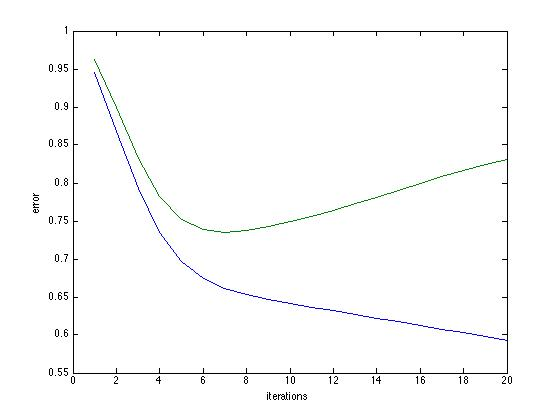
\includegraphics[width=0.7\textwidth]{3b.jpg}
\caption{\label{fig:errors} Number iterations (contractive map was ran) vs the avg. errors. Upper (green) curve is test error and the lower(blue) curve is training error.}
\end{figure}

 See figures/plots. My toy dataset was pest 1 data. Sigma was the average distance between points 0.528 as instructed on the question. Similarly, the test set sigma was for test set was 0.533.

From my plot it is clear that early stopping at around 6 or 7 iterations can achieve a better generalization error, because, its where the error for the test set is the lowest and also, where the training error is not to low (but neither to high that overfitting has occurred).


c) First, let's show that if $c_{\lambda}^* = T(c_{\lambda}^*)$  then it minimizes the Tiknhonov regularization.
If $ c^* = T(c^*) $ 
$$ c^* = c^* - \frac{1}{n+\lambda}(Kc^*+\lambda Ic^*-Y) $$
$$ Y - Kc^* = - \lambda Ic^* $$

Now,lets show that the above $c^*$ minimizes the empirical risk:

$$ J(c) = \|Y-Kc\|_2^2 + \lambda c^t K c $$
$$ \bigtriangledown_c J(c) = -2K(Y-Kc) + 2\lambda K c $$

Now lets substitute $Y-Kc^* = \lambda I c^*$ in the gradient of $J(c)$:

$$\bigtriangledown_c J(c^*) = -2K(Y-Kc^*) + 2\lambda K c  = -2K(\lambda I c^*) + 2\lambda K c^* = - \lambda K c^* + \lambda K c^* = 0 $$

Which concludes our proof. i.e. we proved that $\hat{c}$ minimizes the empirical risk. \\

Now, Let's prove the converse. Given a minimizer $\hat{c}$ of $J(c)$ (empirical risk), then we have a fixed point of the contractive map i.e. $T(\hat{c}) = \hat{c}$.

$$ \bigtriangledown_c J(c) = -2K(Y-Kc) + 2\lambda K c = 0 $$
$$ c = (K^2 + \lambda K)^{-1}KY = (K(K + \lambda I))^{-1}KY = (K + \lambda I)^{-1}K^{-1}KY $$
$$ c^* = (K + \lambda I)^{-1} Y $$

Now, lets substitute $\hat{c}$ in contractive map,

$$ T(\hat{c}) = (K + \lambda I)^{-1} Y - \frac{1}{n+\lambda}((K + \lambda I)(K + \lambda I)^{-1} Y-Y) = (K + \lambda I)^{-1} Y - \frac{1}{n+\lambda}(Y-Y) $$
$$ (K + \lambda I)^{-1} Y = \hat{c}$$

Similarly, this argument holds if $(K + \lambda I)^{-1}$ exists and $\lambda \neq 0$. However, for Tikhonov regularization, $\lambda \neq 0$, thus converse is always true. Which completes our iff proof! Hence, $c_{\lambda}^*$ solves Tikhonov if and only if it also satisfies $c_{\lambda}^* = T(c_{\lambda}^*)$ with the contractive map given in the question. \\

d) See figures/plots.

\begin{figure}
    \centering
    \begin{subfigure}[b]{0.3\textwidth}
        \centering
        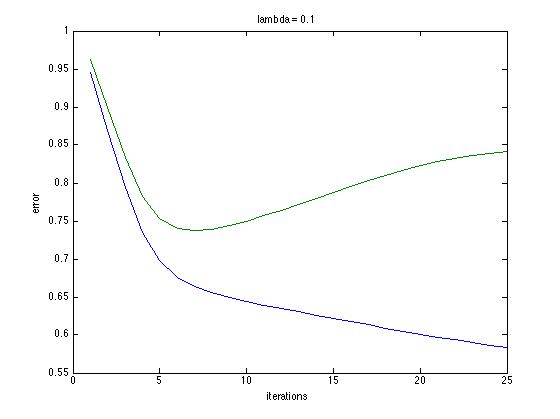
\includegraphics[width=\textwidth]{l01.jpg}
        \caption{$\lambda = 0.1$}
        \label{fig:y equals x}
    \end{subfigure}
    \hfill
    \begin{subfigure}[b]{0.3\textwidth}
        \centering
        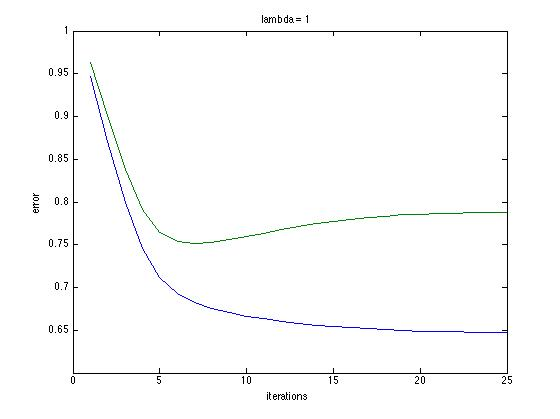
\includegraphics[width=\textwidth]{l1.jpg}
        \caption{$\lambda = 1$}
        \label{fig:three sin x}
    \end{subfigure}
    \hfill
    \begin{subfigure}[b]{0.3\textwidth}
        \centering
        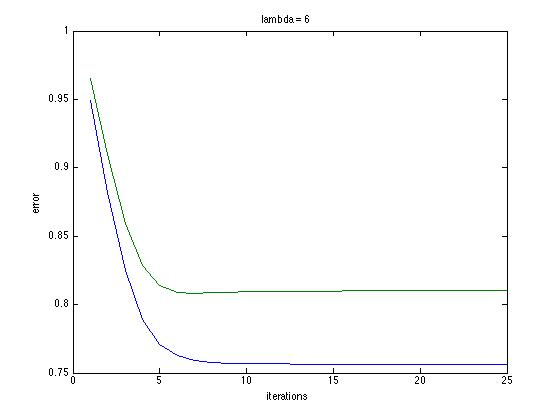
\includegraphics[width=\textwidth]{l6.jpg}
        \caption{$\lambda = 6$}
        \label{fig:five over x}
    \end{subfigure}
    \caption{Comparing three values of lambda and iterations.}
    \label{fig:3d}
\end{figure}

From the plots I provided we can appreciate that with a higher regularization parameter, we would get a more "flat" region where the test error didn't really change anymore even if we ran more iterations of our update rule. For smaller values of lambda,the plot was more similar to the one I provided in part b (obviously, to be expected). I think that the regularization parameter actually acted as an "extra force" to avoid overfitting. Basically, because of the regularization parameter, we could be more carless on the early stopping because after a while, the curve simply evened out. Therefore, we could run more interations of our contractive map with a lower risk of overfitting. Basically, $\lambda$ was already fighting the force of us choosing a highly complex function and not truly learning from the data. Therefore, running extra iterations of $T(c)$ had a lower change of overfitting. Also, as we had a higher lambda, the test error tended to be smaller for the three plots I provided. 

%%%%%%%%%%%%%%%%%%%%%%%%%%%
\paragraph{Problem 4}
%%%
a)Theorem: Given the conditions in the question, the the upper bound we are looking for is as follows:

$$Pr[ \sup\limits_{f \in \mathcal{H}}  | I_s[f] - I[f] | \geq \epsilon] \leq \frac{N(c^2-2cM+M^2)^2}{n \epsilon^2}$$
\begin{proof}
If the largest difference between the empirical risk and the expected risk is larger than $\epsilon$, then that means at least one the defect is larger than $\epsilon$. i.e.:

$$Pr[ \sup\limits_{f \in \mathcal{H}}  | I_s[f] - I[f] | \geq \epsilon] \leq Pr[\cup^{N}_{i=1} | I_s[f_i] - I[f_i] | \geq \epsilon] $$

by the union bound:

$$Pr[ \sup\limits_{f \in \mathcal{H}}  | I_s[f] - I[f] | \geq \epsilon]  \leq \sum^{N}_{i=1} Pr[| I_s[f_i] - I[f_i] | \geq \epsilon] $$

By chevychev's (since we known $\mathbb{E}[I_s[f]] = I[f]$) we have:

$$ Pr[ | I_s[f_i] - I[f_i] | \geq \epsilon] \leq \frac{ Var[X_i] }{ \epsilon^2 } \implies \sum^{N}_{i=1} Pr[| I_s[f_i] - I[f_i] | \geq \epsilon] \leq \sum^{N}_{i=1} \frac{ Var[I_s[f_i]] }{ \epsilon^2 }$$

Now if we can upper bound the variance, we are done.

$$ Var[I_s[f_i]] = Var[\frac{1}{n} \sum^n_j V(f_i,z_j)]$$

Since the function $f_i$ is fixed (i.e. NOT chosen based on the S) and the only randomness involved is with selecting samples/data from z, then the cost functions are iids thus:

$$ Var[\frac{1}{n} \sum^n_j V(f_i,z_j)] = \frac{1}{n^2} \sum^n_j Var[V(f_i,z_j)] = \frac{1}{n}Var[V(f_i,z_j)]  $$

$$Var[V(f_i,z_j)] = \mathbb{E}[V(f_i,z_j)^2] - \mathbb{E}[V(f_i,z_j)]^2$$

To upper bound the above we need to upper bound $\mathbb{E}[V(f_i,z_j)^2]$ and lower bound $\mathbb{E}[V(f_i,z_j)]^2$. 

It is easy to lower bound $\mathbb{E}[V(f_i,z_j)]^2$ because it is the squared loss function, which can never be less than zero. Therefore, the lower bound is $\mathbb{E}[V(f_i,z_j)]^2 \geq 0$.

To upper bound  $\mathbb{E}[V(f_i,z_j)]^2$ we need to substitute in the definition of the squared loss function $\mathbb{E}[V(f_i,z_j)^2] = \mathbb{E}[f_i(x)^2 - 2f_i(x)y + y^2] $. Since $sup_x \in X |f(x)| \leq C$ and the max value of any y is $M$, then we have:

$$\mathbb{E}[V(f_i,z_j)^2] \leq \mathbb{E}[(C^2 - 2CM + M^2)^2] = (C^2 - 2CM + M^2)^2 $$

Setting the terms to be their max value and min value respectively, we get:

$$Var[V(f_i,z_j)] = \mathbb{E}[V(f_i,z_j)^2] - \mathbb{E}[V(f_i,z_j)]^2 \leq (C^2 - 2CM + M^2)^2 - 0 = (C^2 - 2CM + M^2)^2$$

$$Var[I_s[f_i]] \leq \frac{1}{n} (C^2 - 2CM + M^2)^2$$

$$ \therefore Pr[ \sup\limits_{f \in \mathcal{H}}  | I_s[f] - I[f] | \geq \epsilon] \leq \sum^{N}_{i=1} \frac{ Var[I_s[f_i]] }{ \epsilon^2 } = \sum^{N}_{i=1} \frac{1}{n} \frac{ (C^2 - 2CM + M^2)^2 }{ \epsilon^2 } = \frac{N}{n} \frac{ (C^2 - 2CM + M^2)^2 }{ \epsilon^2 }$$
\end{proof}
%%%

b) Let $f_s = argmin_{f \in \mathcal{H}} I_s[f]$, i.e. the minimizer of the empirical risk. Then obviously the defect wrt to this the minimizer of the empirical risk is upper bounded by the probability from the previous part of the question, i.e.

$$Pr[| I_S[f_s] - I[f_s] | \geq \epsilon|]= Pr[ \sup\limits_{f \in \mathcal{H}}  | I_s[f] - I[f] | \geq \epsilon] \leq \sum^{N}_{i=1} Pr[| I_s[f_i] - I[f_i] | \geq \epsilon] \leq \frac{N(c^2-2cM+M^2)^2}{n \epsilon^2}$$

The difference btw generalization and empirical error is either above epsilon or bellow it:

$$1 - Pr[| I_S[f_s] - I[f_s] | \leq \epsilon ] = Pr[| I_S[f_s] - I[f_s] | \geq \epsilon] \implies Pr[| I_S[f_s] - I[f_s] | \leq \epsilon ] \geq 1- \frac{N(c^2-2cM+M^2)^2}{n \epsilon^2} $$

If we want to have at least $1 - \eta$ confidence that the empirical error will be $\epsilon-$close to the generalization error the equation bellow must hold:

$$Pr[| I_S[f_s] - I[f_s] | \leq \epsilon ] \geq 1- \frac{N(c^2-2cM+M^2)^2}{n \epsilon^2} \geq 1- \eta$$

Therefore, the closeness holds (i.e. above inequality) holds if the following holds:

$$1- \frac{N(c^2-2cM+M^2)^2}{n \epsilon^2} \geq 1- \eta \implies \epsilon \geq \sqrt{\frac{N(c^2-2cM+M^2)^2}{n \eta}}$$

Therefore, that means that the difference between the true generalization error and the empirical risk is at most $\sqrt{\frac{N(c^2-2cM+M^2)^2}{n \eta}}$ with $1 -\eta$ confidence:

$$| I_S[f_s] - I[f_s] | \leq \epsilon | \geq \epsilon = \epsilon(n, \eta, N) =   \sqrt{ \frac{N(c^2-2cM+M^2)^2}{n \eta} } $$

With the the absolute value function we have $I_s[f_s] - I[f_s] \leq e(n, \eta, N)$ and $I[f_s] - I_s[f_s] \leq e(n, \eta, N) $ are true. Since we are interested in bounding the generalization error we will be interested in the second inequality.Thus:

$$I[f_s] - I_s[f_s] \leq \epsilon(n, \eta, N) \implies I[f_s] \leq I_s[f_s] + \epsilon(n, \eta, N) =  I_s[f_s] + \sqrt{ \frac{N(c^2-2cM+M^2)^2}{n \eta} }$$

As $N = |\mathcal{H}|$ increases, then that means the we are increasing the space of functions we are allowing ourselves to choose from. Since we are adding more functions to choose from without removing previous functions we already had in $\mathcal{H}$, the empirical risk cannot increase. If this is true, then the empirical risk can only decrease. This means that $I_S[f_S]$ can only decrease as $N$ increases. So we might get a lower empirical risk. 

However, as N increases, $\epsilon(n, \eta, N)$ increases wrt to the growth of  the square root of N . Meaning that our difference between empirical and generalization error becomes more lose, in the sense that the upper bound increases. This is not good because if N becomes very large, then the event that we are trying to impose a probability, will become less and less interesting. To illustrate my argument, take as an extreme case, if $\epsilon(n, \eta, N) = \infty$, then we are trying to impose an upper bound on the probability that the empirical risk is really far from the generalization. However, if we allow the difference to be infinity, then it becomes an uninteresting probabilistic event, even if we know the probability exactly. i.e. we know for sure that their difference will be less than infinity if both are finite real numbers.

Now lets explore the sum of them $I_S[f_S] + \epsilon(n, \eta, N)$. As N increases $I_S[f_S]$ can only decrease and $\epsilon(n, \eta, N)$ increases for sure. However, $I_S[f_S]$ doesn't necessarily have to decrease for every unit of N that we increase, while $\epsilon(n, \eta, N)$ for sure increases for every unit of N. This makes overfitting more likely. As N increases $I_S[f_S]$ \textbf{might} decrease, however, we know for sure that $\epsilon(n, \eta, N)$ increases. This gives us an upper bound on $I[f_S]$ (generalization error) that increases most of the times as $N$ increases. This means that our upper bound estimate for the generalization error becomes more and more useless and that the empirical error becomes less good as a proxy for $I[f_S]$. Thus, yielding overfitting more and more likely.

4c)

\begin{proof}

If we want with $1 - \eta$ confidence that the generalization and empirical error are close, then from ideas explained in part b the following equation holds:

$$ | I[f_s] - I_s[f_s] | \leq \epsilon(n, \eta, N)$$

and

$$ | I[f^*] - I_s[f^*] | \leq \epsilon(n, \eta, N)$$

Therefore we know that:

$$ I[f_s] - I_s[f_s] \leq \epsilon(n, \eta, N)$$

and

$$ I_S[f^*] - I[f^*] \leq \epsilon(n, \eta, N)$$

Add the above two inequalities:

$$I[f_s] - I_s[f_s] +  I_s[f^*] - I[f^*] = (I[f_s] - I[f^*]) + (I_S[f^*] - I_s[f_s])  \leq 2\epsilon(n, \eta, N)$$

The second expression in brackets is greater than or equal to zero i.e. $I_s[f^*] - I_s[f_s] \geq 0$. This is because $f_s$ is chosen such that it minimizes the empirical risk. Therefore, there cannot be any function that achieves a lower empirical risk that the minimizer of the empirical risk. Therefore:

 $$I_S[f^*] \geq I_s[f_s] \implies I_S[f^*] - I_s[f_s] \geq 0$$
 
 Therefore we know that $I[f_s] - I_s[f_s] \leq (I[f_s] - I[f^*]) + (I_s[f^*] - I_s[f_s]) $. Therefore implying that 
 
 $$I[f_s] - I[f^*] \leq (I[f_s] - I[f^*]) + (I_S[f^*] - I_s[f_s])  \leq 2\epsilon(n, \eta, N)$$
 
  $$I[f_s] - I[f^*] \leq 2\epsilon(n, \eta, N)$$
 
 As required.

\end{proof}

%%%
\paragraph{Problem 5 (MATLAB)}
a) Code
b)Code
C) When we plotted the accuracy on the unlabeled data against n (the number of labeled data) we could see that as n got large, Laplacian and RLS had similar accuracy. However, for smaller values of n, Laplacian had a clear advantage because it was able to incorporate information about the geometric structure of the unlabeled data when. Therefore, when it came around to predict, it had an advantage, because it had information that regular RLS tikhonov had no way of obtaining.

\end{document}

